334.\begin{figure}[ht!]
\center{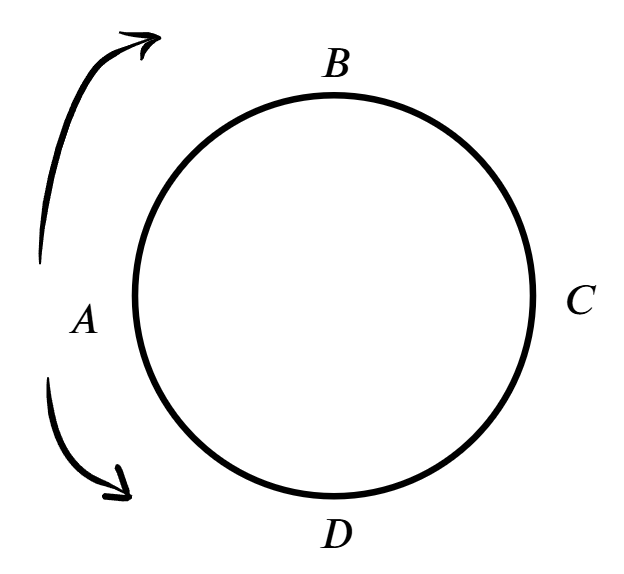
\includegraphics[scale=0.35]{krug3.png}}
\end{figure}\\
Пусть они встречаются в точках $A,\ B,\ C$ и $D.$ Тогда пока первый ездок проезжает дугу $AB,$ второй проезжает дугу $ADCB,$ пока первый проезжает дугу $BC,$ второй проезжает дугу $BADC,$ пока первый проезжает дугу $CD,$ второй проезжает дугу $CBAD$ и пока первый проезжает дугу $DA,$ второй проезжает дугу $DCBA.$ Тогда за то время, пока первый проехал дуги $AB,\ BC,\ CD$ и $DA,$ то есть полный круг, второй проедет дуги $ADCB,\ BADC,\ CBAD,$ и $DCBA,$ то есть три круга. Значит, скорость Максима может быть в три раза больше или в три раза меньше, чем скорость тренера, то есть $12\cdot3=36$км/ч или $12:3=4$км/ч.\\
